\section{Lektion 01-02-2018}

\begin{enumerate}
	\item Lyd i et medium
	\item Hørelsen (opfattet lydniveau)
	\item Ohms lov analogi
	\item Vægtning (filtrering)
	\item Lydens udbredelse (afstandsregel)
	\end{enumerate}

\begin{mdframed}[style=exampledefault]
	\begin{itemize}
		\item \textbf{Pensum:} 
		\begin{enumerate}
			\item Master Handbook Of Acoustics, ch. 1-3
			\item Audio Meetering, sec. 1-6, 11, 13
			\item Elektroakustik, TAS,  p. 6
		\end{enumerate}
		\item \textbf{Opgaver:} 
		\begin{enumerate}
			\item Lyd og Akustik - Lektion 1 - opgaver og øvelser
		\end{enumerate}
	\end{itemize}
\end{mdframed}

\subsection{Lyd i et medium}

\textit{Sound can be viewed as a wave motion in air or other elastic media. In this case,	sound is a stimulus. Sound can also be viewed as an excitation of the hearing	mechanism that results in the perception of sound. In this case, sound is a sensation.}
\begin{itemize}
	\item Lyd er svingning i et medium omkring ligevægt. Uden et medium kan lyd ikke blive udbredt. 
	\item Lyd kan udbredes i medier såsom luft, væsker og materialer af fast form. Lyd kan ikke udbredes i rummet, da mediet her er et vakuum. 
	\item Hvis en luftpartikel bliver forskudt fra dens oprindelig position, vil elastiske krafter forsøge at tilbagevende luftpartiklen til dens oprindelige position.
\end{itemize}

\begin{figure} [H]
	\centering
	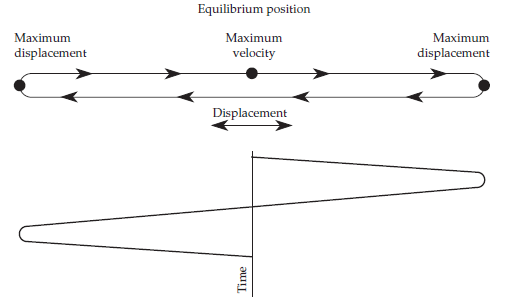
\includegraphics[width=0.85\linewidth]{graphics/1.png}
	\caption{En luftpartikel der vibrerer rundt om dens medie som er i ligevægt (elastiske krafter).}
	\label{fig:1}
\end{figure}

\begin{itemize}
	\item Fluktationerne i trykket omkring det atmosfæriske tryk er meget små.
	\begin{itemize}
		\item Normal tale ses som små ripples i det atmosfæriske tryk.
		\item Den mindste ændring i trykket et øre kan opfatte er således \SI{20}{\micro\pascal}. Dette svarer til et tryk der er 5 millioner gange mindre end det atmosfæriske tryk.
	\end{itemize}
	\item Lydens hastighed er $c = \SI{344}{\meter\per\second}$
	\begin{itemize}
		\item Lydens udbredelse (hastighed) afhænger af mediets densitet.
		\begin{itemize}
			\item Jo større densistet, jo nemmere er det for partiklerne at overføre energi. Lyd udbredes derfor hurtigere i væsker og materialer i fast form end i luft.
		\end{itemize}
		\item Lydens udbredelse afhænger også af temperatur og luftfugtighed.
		\begin{itemize}
			\item Jo højere temperatur, jo hurtigere udbredes lyden. 
			\item Jo højere luftfugtighed, jo hurtigere udbredes lyden.
		\end{itemize} 
	\end{itemize}
\end{itemize}

\begin{figure} [H]
	\centering
	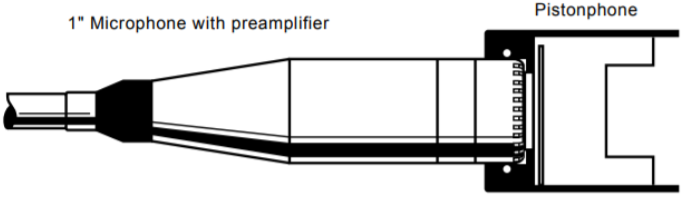
\includegraphics[width=0.85\linewidth]{graphics/2.png}
	\caption{(A) Variationer af luftryk komprimerer luftpartiklerne. \\(B) Variationerne ligger lige over og lige under det atmosfæriske tryk. }
	\label{fig:2}
\end{figure}

\begin{itemize}
	\item Bølgelængde og frekvens
	\begin{itemize}
		\item Frekvens (waveform repitions per unit of time) 
	\end{itemize}
\end{itemize}
\begin{equation}\label{eq:freq}
f = \frac{c}{T}
\end{equation}
\begin{itemize}
	\item 
	\begin{itemize}
		\item Wavelength (to complete one cycle) 
	\end{itemize}
\end{itemize}
\begin{equation}\label{eq:wave}
T = \frac{c}{f}
\end{equation}

\subsection{Hørelsen}
\begin{itemize}
	\item Tonehøjden (pitch) af en frekvens høres forskelligt af øret.
	\item Tonehøjden for en \textbf{lav frekvens dæmpes} når intensiteten øges mens tonehøjden for en \textbf{høj frekvens øges} når intensiteten øges.
	\item Harmonisk er en lineær skala.
	\item Oktaver er en logaritmisk skala ofte anvendt i musik fordi den skalerer bedre til ørets opfattelse af lyd. 
	\begin{itemize}
		\item En oktav er defineret ved en 2:1 ratio af to frekvenser. 
		\item Intervallet fra \SI{100}{\hertz} til \SI{200}{\hertz} opfattes som værende større end intervallet fra \SI{200}{\hertz} til \SI{300}{\hertz}. 
	\end{itemize}
\end{itemize}

\begin{figure} [H]
	\centering
	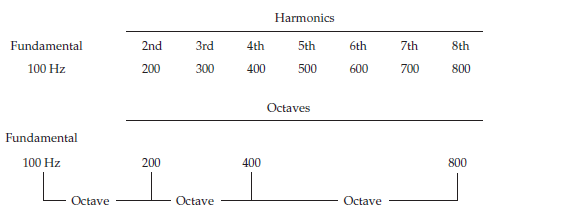
\includegraphics[width=\linewidth]{graphics/3.png}
	\caption{Sammenligning mellem harmoniske og oktaver. }
	\label{fig:3}
\end{figure}

\begin{equation}\label{eq:octave}
\frac{f_2}{f_1} = 2^n
\end{equation}

\begin{description}
	\item $f_2$ = frequency of the upper edge of the octave interval, \si{\hertz}
	\item $f_1$ = frequency of the lower edge of the octave interval, \si{\hertz}
	\item $n$ = number of octaves
\end{description}

\begin{itemize}
	\item Scopet af det hørbare spektrum er \SI{20}{\hertz} til \SI{20}{\kilo\hertz}.
	\begin{itemize}
		\item Der er lyde der ikke kan høres af øret. Det er frekvenser der er lavere end det hørbare spektrum (infrasound) og frekvenser der er højere end det hørbare spektrum (ultrasound).
	\end{itemize}
	\item Intensiteten af lyden $I_L$ kan opgives i decibel [dB] ved at anvende reference $I_{ref} = \SI{20}{\micro\pascal}$ som er den mindste ændring i trykket et øre kan opfatte.
	\item Lydeffekten kan ligeledes opgives i \si{\decibel}ved at anvende reference effekt $L_p = \SI{1}{\pico\watt} = 10^{-12} \si{\watt}$.
\end{itemize}

\begin{equation}\label{eq:decibel}
PW_L = 10\log_{10}\frac{W}{W_{ref}}
\end{equation}

\begin{description}
	\item $PW_L$ = sound-power level, \si{\decibel}
	\item $W$ = sound power, watts
	\item $W_{ref}$ = a reference power, $10^{–12}$ \si{\watt}
\end{description}

\begin{figure} [H]
	\centering
	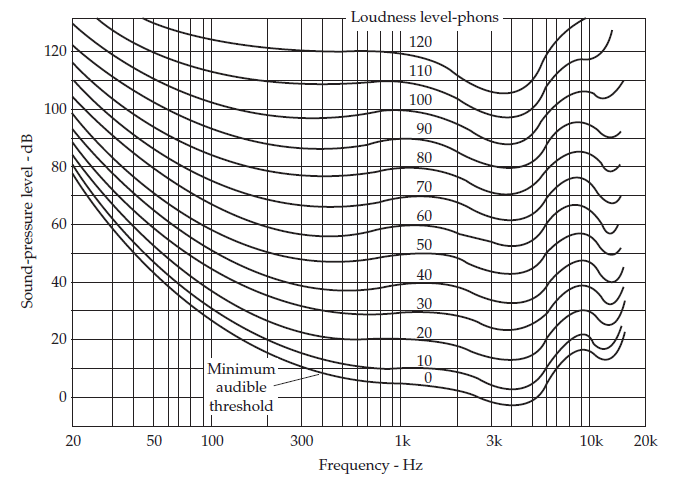
\includegraphics[width=\linewidth]{graphics/8.png}
	\caption{Det menneskelige øres opfattelse af subjektivt konstant lydtryk.}
	\label{fig:8}
\end{figure}

\begin{itemize}
	\item Lydintensitet er svært at måle. Men lydtryk (sound pressure level $SP_L$) er derimod det nemmeste at måle. Derfor anvendes lydtryk ofte.
	\begin{itemize}
		\item $SP_L$ er tæt på at være ens med $I_L$, hvor begge ofte bliver referet til som lydniveauet (sound level).
	\end{itemize}
\end{itemize}

\begin{equation}\label{eq:spl}
SP_L = 20\log_{10}\frac{p}{p_{ref}}
\end{equation}

\begin{description}
	\item $SP_L$ = sound-pressure level, \si{\decibel}
	\item $p$ = acoustic pressure, \si{\micro\pascal} or other
	\item $p_{ref}$ = acoustic reference pressure, \si{\micro\pascal}  or other
\end{description}

\begin{figure} [H]
	\centering
	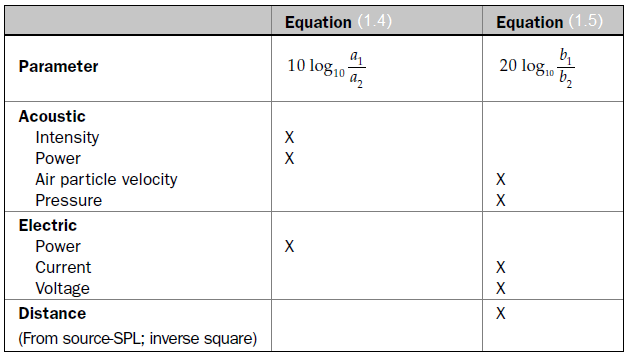
\includegraphics[width=\linewidth]{graphics/6.png}
	\caption{Om der skal bruges 10 log og 20 log. }
	\label{fig:6}
\end{figure}

\begin{itemize}
	\item Når effekten fordobles svarer det til en \SI{3}{\decibel} forøgelse uanset om effekten fordobles fra \SI{1}{\watt} til \SI{2}{\watt} eller fra \SI{100}{\watt} til \SI{200}{\watt}.
\end{itemize}

\subsection{Ohms lov analogi}
\begin{itemize}
	\item Et akustisk system som en højtaler kan blive repræsenteret i termer der er ækvivalente med et elektrisk eller mekanisk system. 
\end{itemize}

\begin{figure} [H]
	\centering
	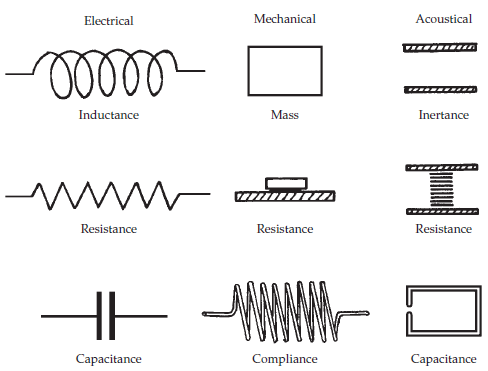
\includegraphics[width=0.5\linewidth]{graphics/4.png}
	\caption{De 3 basale elementer af elektriske systemer og deres analogier i mekaniske og akustiske systemer.}
	\label{fig:4}
\end{figure}

\begin{figure} [H]
	\centering
	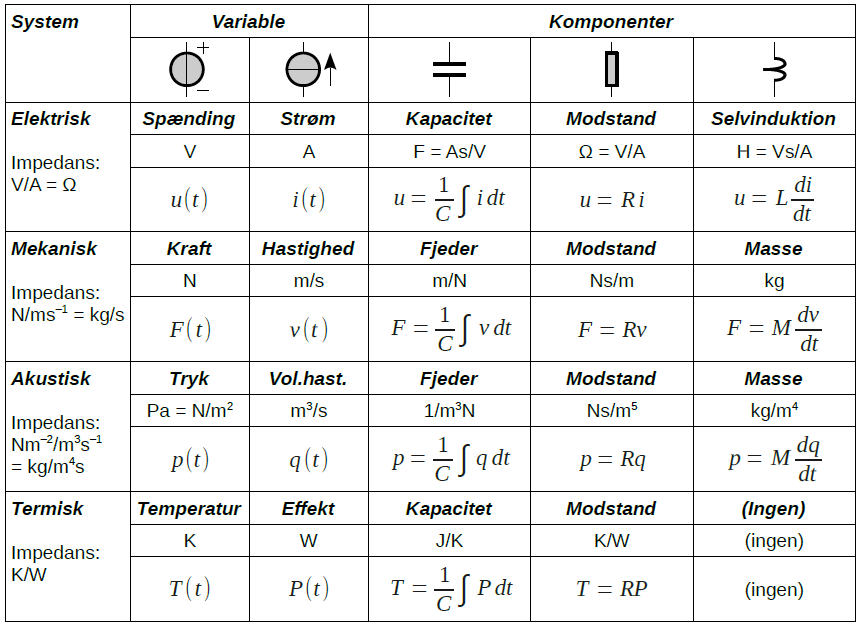
\includegraphics[width=\linewidth]{graphics/5.png}
	\caption{Analogier for komponenter i et elektrik, mekanisk og akustisk system.}
	\label{fig:5}
\end{figure}

\subsection{Vægtning}
\begin{itemize}
	\item Ved måling af lydtryk benyttes ikke blot en mikrofon og en forstærker. Hørelsen er kompleks og for at efterligne hjernens opfattelse af et lydniveau benyttes nogle elektriske filtre
	\item Filtrene A, B og C modificerer frekvensresponsen så den efterligner hørekurven ved lavt, middel og højt lydniveau.
	\begin{itemize}
		\item A-vejning korrelere godt til nedslidningen af hørelsen ved kraftige signaler og benyttes derfor ved støjmåling.
		\item B-vejning benyttes ikke mere.
		\item C-vejning bruges til specifikation af kortvarige spidser for måling af støjens skadevirkning ved klassifikation af en arbejdsplads for påbudt brug af høreværn.
	\end{itemize}
\end{itemize}

\begin{figure} [H]
	\centering
	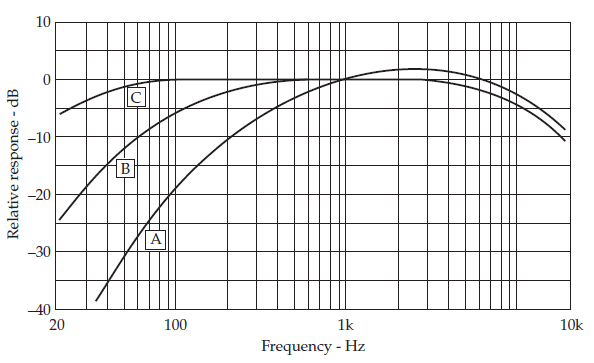
\includegraphics[width=\linewidth]{graphics/7.png}
	\caption{A, B, and C weighting response characteristics for sound-level meters.}
	\label{fig:7}
\end{figure}

\begin{description}
	\item For sound-pressure levels of 20 to 55 dB, use network A.
	\item For sound-pressure levels of 55 to 85 dB, use network B.
	\item For sound-pressure levels of 85 to 140 dB, use network C.
\end{description}


\subsection{Lydens udbredelse}

\begin{itemize}
	\item Punktlydkilde: Lyden udbredes ligeligt i alle retninger.
	\begin{itemize}
		\item Lyden fra en punktlydkilde ændrer \textbf{ikke} udseende ved stigende afstand.
		\item En plan lydbølge er en matematisk abstraktion og følgende tilnærmelser anvendes:
		\begin{itemize}
			\item Lydens udbredelse i smalle rør (musikinstrumenter, fjernvarme).
			\item Lydens udbredelse i stor afstand fra lydkilden.
			\item Højttalerens nærfelt.
		\end{itemize}
	\end{itemize}
\end{itemize}

\begin{figure} [H]
	\centering
	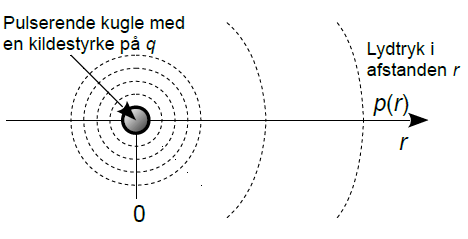
\includegraphics[width=0.65\linewidth]{graphics/9.png}
	\caption{Lyden fra en punktkilde udbredes fra kildens centrum og lydtrykket aftager ved stigende afstand.}
	\label{fig:9}
\end{figure}

\begin{itemize}
	\item Lydtrykket aftager med stigende afstand idet effekten i den kugleformede bølgefront fordeles over et areal, der vokser kvadratisk med afstanden.
	\begin{itemize}
		\item Nærfelt: Lydtrykket varierer ikke – plane bølger.
		\item Fjernfelt: – \SI{6}{\decibel}/fordobling – sfæriske bølger.
	\end{itemize}
\end{itemize}

\begin{figure} [H]
	\centering
	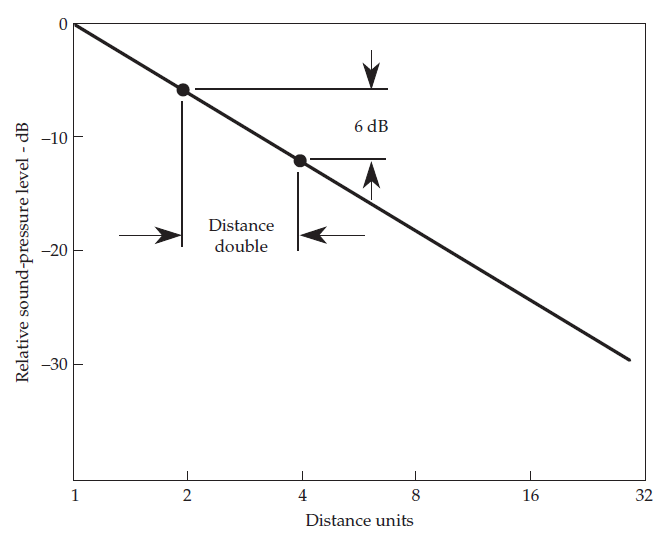
\includegraphics[width=0.85\linewidth]{graphics/10.png}
	\caption{Afstandsregel.}
	\label{fig:10}
\end{figure}

\newpage
\subsection{Opgaver}

\begin{enumerate}
	\item Beregn dB værdien af det maksimalt mulige lydtryk.
	\item Beregn det A-vægtede lydtryk af \SI{76}{\decibel} ved \SI{125}{\hertz}.
	\item Et lydtryk reduceres \SI{8}{\decibel}, hvor mange gange er det?
	\item Hvor meget lydtryk skal der til, for at vi opfatter lyden - ved \SI{63}{\hertz} og ved \SI{2}{\kilo\hertz}?
\end{enumerate}


\begin{lstlisting}
%% LYAK L1 01-02-2018
% 1. Beregn dB vaerdien af det maksimalt mulige lydtryk.
L = 20*log10(10^5/(20*10^-6));
disp(['Det maksimalt mulige lydtryk er ', num2str(L), ' dB']) 

% 2. Beregn det A-vaegtede lydtryk af 76 dB ved 125 Hz.
f = 125;

R_A = (12194^2*f^4)/((f^2+20.6^2)* ...
sqrt((f^2+107.7^2)*(f^2+737.9^2))*(f^2+12194^2));
A = 20*log10(R_A)+2;

disp(['Det A-vaegtede lydtryk af 76 dB (125 Hz) er ', num2str(76+A), ' dB']) 

% 3. Et lydtryk reduceres 8 dB, hvor mange gange er det?
gg = db2mag(8);
disp(['Lydtrykket reduceres 8 dB, hvilket svarer til ', num2str(gg), ' ganges reducering'])
\end{lstlisting}

